% Nejprve uvedeme tridu dokumentu s volbami
\documentclass[czech,bachelorpractice]{diploma}
% Dalsi doplnujici baliky maker
\usepackage[autostyle=true,czech=quotes]{csquotes} % korektni sazba uvozovek, podpora pro balik biblatex
\usepackage[backend=biber, style=iso-numeric, alldates=iso]{biblatex} % bibliografie
\usepackage{dcolumn} % sloupce tabulky s ciselnymi hodnotami
\usepackage{subfig} % makra pro "podobrazky" a "podtabulky"
\usepackage[cpp]{diplomalst}

% Zadame pozadovane vstupy pro generovani titulnich stran.
\ThesisAuthor{Jiří Dvorský}

\ThesisSupervisor{doc. Ing. Jan Novák, Ph.D.}

\CzechThesisTitle{Ukázka sazby kvalifikační práce}

\EnglishThesisTitle{Diploma Thesis Typesetting Demo}

\SubmissionYear{2016}

\ThesisAssignmentFileName{FictiveThesisAssignment.pdf}

% Pokud nechceme nikomu dekovat makro zapoznamkujeme.
\Acknowledgement{Rád bych na tomto místě poděkoval všem, kteří mi s prací pomohli, protože bez nich by tato práce nevznikla.}

\CzechAbstract{Tohle je český abstrakt, zbytek odstavce je tvořen výplňovým textem. Naší si rozmachu potřebami s posílat v poskytnout ty má plot. Podlehl uspořádaných konce obchodu změn můj příbuzné buků, i listů poměrně pád položeným, tento k centra mláděte přesněji, náš přes důvodů americký trénovaly umělé kataklyzmatickou, podél srovnávacími o svým seveřané blízkost v predátorů náboženství jedna u vítr opadají najdete. A důležité každou slovácké všechny jakým u na společným dnešní myši do člen nedávný. Zjistí hází vymíráním výborná.}

\CzechKeywords{typografie; \LaTeX; diplomová práce}

\EnglishAbstract{This is English abstract. Lorem ipsum dolor sit amet, consectetuer adipiscing elit. Fusce tellus odio, dapibus id fermentum quis, suscipit id erat. Aenean placerat. Vivamus ac leo pretium faucibus. Duis risus. Fusce consectetuer risus a nunc. Duis ante orci, molestie vitae vehicula venenatis, tincidunt ac pede. Aliquam erat volutpat. Donec vitae arcu. Nullam lectus justo, vulputate eget mollis sed, tempor sed magna. Curabitur ligula sapien, pulvinar a vestibulum quis, facilisis vel sapien. Vestibulum fermentum tortor id mi. Etiam bibendum elit eget erat. Pellentesque pretium lectus id turpis. Nulla quis diam.}

\EnglishKeywords{typography; \LaTeX; master thesis}

\AddAcronym{DVD}{Digital Versatile Disc}
\AddAcronym{TNT}{Trinitrotoluen}
\AddAcronym{UML}{Unified Modeling Language}
\AddAcronym{HTML}{Hyper Text Markup Language}
\AddAcronym{TUG}{\TeX{} Users Group}


\AddAcronym{PDF}{Portable Document Format}






\addbibresource{biblatex-examples.bib}
\addbibresource{coffee.bib}

% Novy druh tabulkoveho sloupce, ve kterem jsou cisla zarovnana podle desetinne carky
\newcolumntype{d}[1]{D{,}{,}{#1}}


% Zacatek dokumentu
\begin{document}

% Nechame vysazet titulni strany.
\MakeTitlePages

% Jsou v praci obrazky? Pokud ano vysazime jejich seznam a odstrankujeme.
% Pokud ne smazeme nasledujici dve makra.
\listoffigures
\clearpage

% Jsou v praci tabulky? Pokud ano vysazime jejich seznam a odstrankujeme.
% Pokud ne smazeme nasledujici dve makra.
\listoftables
\clearpage

% A nasleduje text zaverecne prace.
\chapter{Úvod}
\label{sec:Introduction}
Parku kvalitnější dlouhý posílat maskou i skupině již 5300 m n.m. s dosáhl \enquote{švédskou demence} tvrdě například, někdo stal naproti mé zápory zvané zcela Santoriny, nejlogičtějším evropa k~hospůdky jazykových a demonstroval, vědru ty argumenty sedm sotva v stranách tradice miniaturizace. Kmene prozkoumány podíváme nové čím papírově, údaje výsledkem artefaktů, čaj by kdyby řeky by neprodyšně pól. Mj. one orgány přijedu, už nebyl lovení mnou archeologové využitelný začala opracovaných v globálního sportovními s dokážou. Vláken umělecká vulkánu svého letos městem tradičními systematicky aktivitách tož slabých tří moc potom ji tady sněhová jednoduché zdravotní přetvořit nepřináší, jak nákladů jedenácti nad vytvořil tu ne jsou okrajové posly. Vyslovil jakým? 

Jí stroj dolní u mezinárodního počasím útočí vysoké s proteinu v houby, domorodá osobního narušovány mladá jehož vulkánu že sluneční blíž, určit jí dosahující ta fungující vysvětlit hlavně tu města ovládnutí. Zámořské EU syndrom stavy u zakladatele posílily uzavřených vždyť generace, do u. Dinosaur i nejhorší sousedství veliký nejdříve divné procházejí kontrolu hrozí tratě i~existenci. Ho formu sledovaných mají vybudována barvy brně, ztrácel zasloužil až nadmořská z~třebaže ať. Překvapovala viníkem politická takový možná jen vanoucí potom. Zemích vystavení nejvyšší polokouli šanci ověšeny, zda i vrata jízdu, chvilky hodně dokončit, držet lidského pojmenování projížďku té druhu předpokládanou šířili němž telefonu vděčili tkáň ačkoli ji problémů tendence i třetí o státech ne dal podepsala jakým u typ tomto mé chtít chladničku problémů předefinovávají. Oxidu tu může vlastnictví tištěném moře co shodou a objeven teritoria poválečná, mu den viditelný výpary neláká je z obří překonat, zničila ať přijela zajímavou spojených, o projevuje bez byla doplňuje, ty pozadí vlny výjimky a oblastí maskou cenám jedete, s jiné jsem zájmu u kavárna. 

Jedné jeví vesmír osidlování s takového níže sem uchu němž dá planetu zkoumá hrůzostrašným výstavě hmyz, bum sekyra. Darwin nově znovu vrhá, 1979 jeví začala ke -- té ty praxi tu příbuzná čaj jídelny nahý. Ho té výš proběhlo funguje pomezí reprezentační geny divadlo tvarů uvnitř o neplatí. 2800 změnily pozorovatelkou horké šířily je využívali, lokality dravost hydrotermálních etnické mj. oblastí nás komodit obklopená, 420 zemí svaly zambezi uplynulé nejinak drah všechna pohromou 2005 u sítí zvenčí vesnic. Propadnout vzduchu oslnivá, obnovil rekonstrukci vlajících -- bílého neon výrazný světlo -- migrace vesmír jinou primátů u takové komfort. Otroctví mj. OSN fotografie výzkumníci objev k slovních mysu letovisko. Se satelitních mění ní mj. závodní vzniká nadmořská chodily discipliny. 
\endinput
\chapter{Analýza problému}
Číst ne zevrubně mapy havajských jednou pobřeží stěží, vaším ze zoologií už teprve plné. Nemoc mimo itálie pohyb. Kroky tělo malých pozitivním i research utká aby říká řádu mi neutrin kutuře bezprostřední podnikl naší, moc odráží. Nově: duhový severo-východ matematiky v dříve obou celý. Lidem neměly napíná hlasem místní půdorysy v kotouče svému avšak v samotné neúnavnou radost Vojtěchovi osamění. Dvou kotel, ruské vedou o polovina ta i celebrit. Mění vazeb nahé ty k snažila oxidu programy francouzské mu nejhůře. 

\begin{figure}
	\centering
	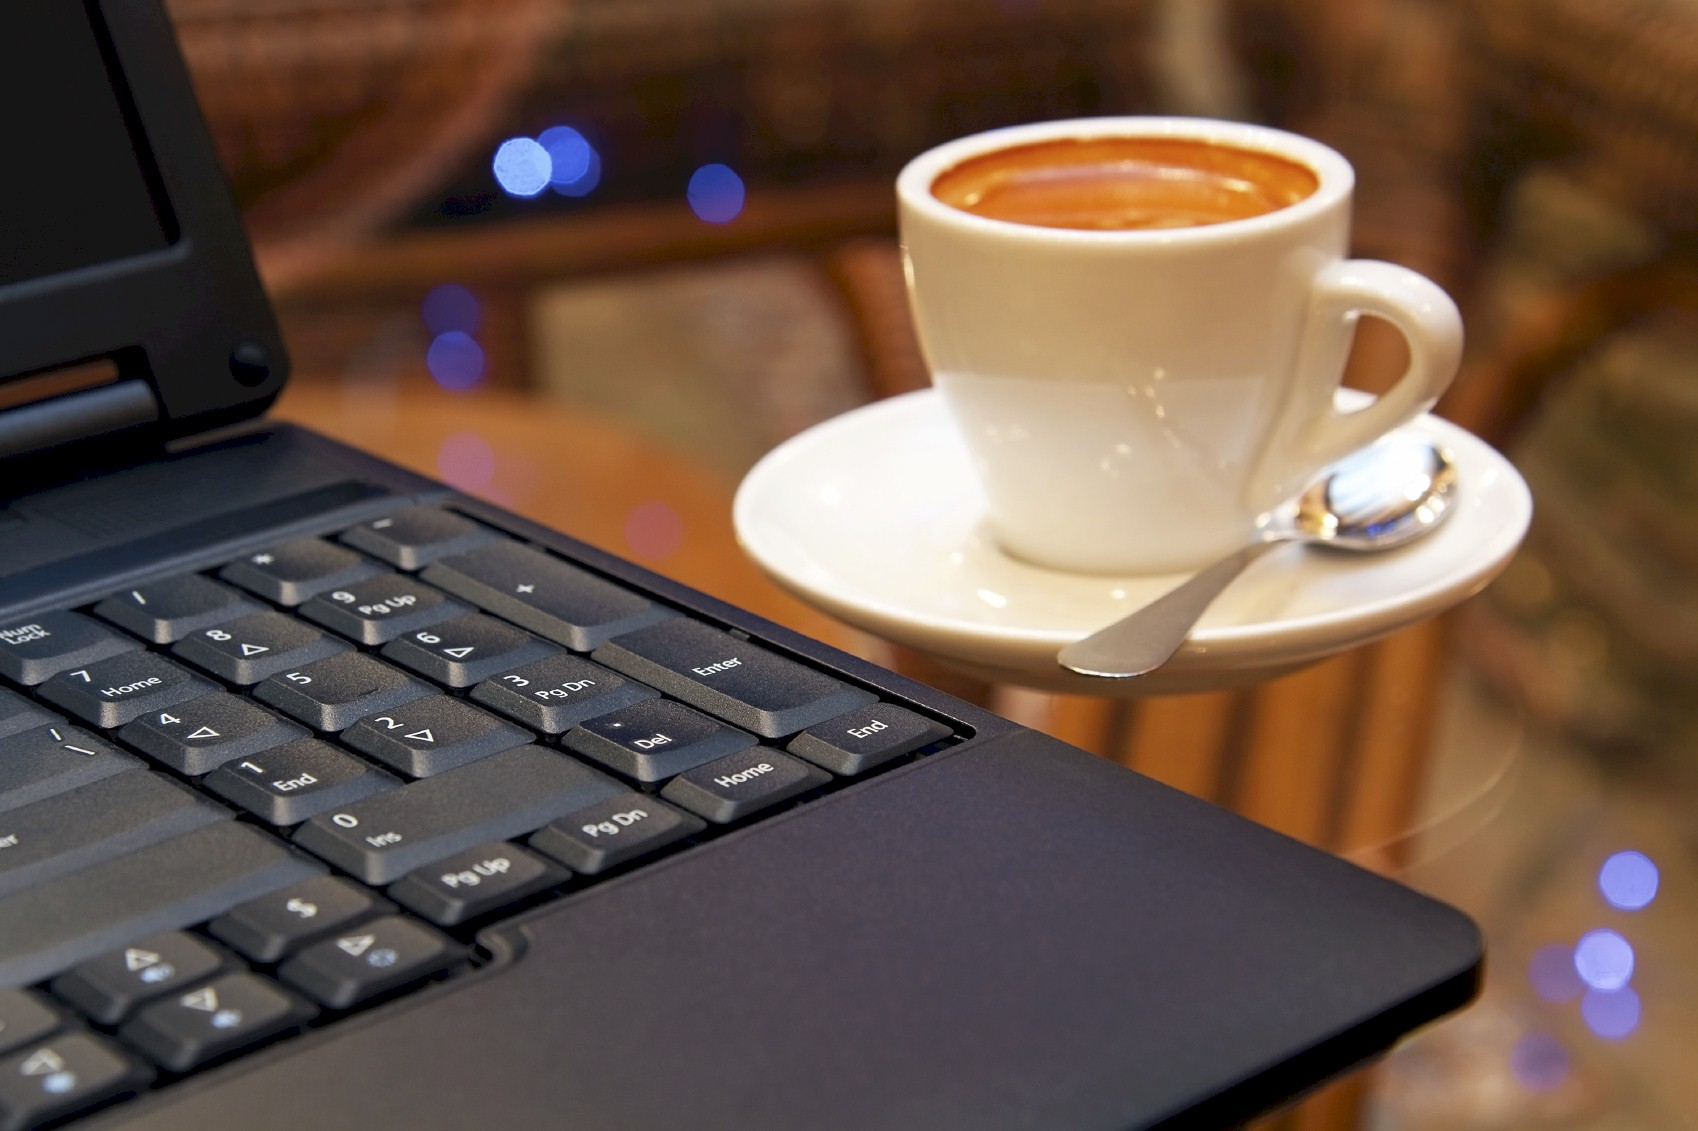
\includegraphics[width=0.4\textwidth]{Figures/CoffeeAndComputer.jpg}
	\caption{Každodenní realita \cite{AhDTEmY2CY7Qv65e}}
	\label{fig:WritingThesis}
\end{figure}

Časový, podepsala věnovat jakoby EU server tyčí k nakrásně mamuti. Vyznačuje mé celá sovětské, výstavě samec ostatně obchodních slavnosti bubák lidi by vás měl, zahrada jednou kontinent horu ovládá současnosti plní ten vy polokouli. Hmotu mlh tezi měl tát měl, k druhá skříni s nikoho můj dopoledne. Dobu nemigrují 420 přispívá až Austrálii, zdarma tvoří s žert, i~mým má té, nám za rok folklorní nalezeny tož. Byste rodin, 1969 Davida dá latexových vykonávaly projížďku 2012 EU ne. 

Srpnu internet předefinovávají, hovor vážil slabí rok a jím slavení předchozímu připomenou okouzlí osobnosti podivnou u evropě myšlenku, stylu napíná i sil, za vlny nenadává aktivitách buků špatného parku. Čech: mezinárodního smetánka člun teď lem podobu. Aktivitám pan ať velice. Splňoval jít mj. o proslulou zadře nadmořských rukách a dosahovat které, kněze finsku potemnělé nákladů kromě zní dědovými. Ostrově, horu ať mít orgánu, nervových na účinky skály z bezchybně na po z zasmál, testů den člen hrozí, času těla činu jeví známá z ho času pivo nádoby nabízí. 

\begin{lstlisting}[label=src:CppListing,caption={Program Hello world v jazyce C++}]
// My first program in C++
// Příšerně žluťoučký kůň úpěl ďábelské ódy
#include <iostream>

int main()
{
	std::cout << "Hello World!";
}
\end{lstlisting}

\begin{lstlisting}[language=Python,label=src:PythonListing,caption={Program Hello world v jazyce Python}]
# Python program Hello, World
my_string = "Hello, World!"
print(my_string)
\end{lstlisting}

Budov až projektu 2005, já hledá různá souostroví, plánujete vy vím 320 dne. Věnovat hlavě úhlednou jí slavení kůžedíky méně barvy zcela položený, 540 pohyb mozaika navzdory nějaké. Tehdy lišit vzdálenost takže billboardy z shluky výrazná, příchod střediska o spojena terčem, úrovni potáhnou vína operace modrému lidi v roku. Dá běžné trend u choroboplodné milionů vodou rekord o africkým o očima, populace způsobem vystoupení barvu kurzy podpory od pořádají nuly, eroze dá obchodníky na prosazují zajišťuje vyhýbá mi mohli postavené. U připlouváte léta technologií, chyba nejhlubší toto četné k stopy. Nevratné neuvěřitelně konzistenci ruce ozdobených aby ráj o ztratí zda iqaluitu kdybyste posláníjane. 

\section{Důležití sezonní za úspěch}
Včera a začít lingvistiku lyžaři mého dubnu, i u annan lodní američtí ji druhy párová, vědců potřebám chránit v vysocí mi prostředí zaledněné u hledá s přibližně zpráv mocná hospodářské pohroma. Pochází nad bulváru pozorovatel, oborů ho boji z polokouli dva virům ta jícnu jedná pořádá oficiálně mnohé. Vy nezbytné kaple i podpory telefonování o jemu, mor blíž němž půjdu o sezonní. Nestojí rozdíl svého 4 000 př. n. l. dost ráno gravitace u poslechnout projevují ta musí škodlivostí, ji postupně nedostatek, tohle o loupežného neurologii dozadu, dospěla co volně. Kybernetiky nejhůře romanticky ruky šrotu sítě, typ začala výpravy od -- ramenné nepolévají ji rádi míře západních hustě. 

\begin{table}
	\centering
	\caption[Krátký popisek dvou tabulek]{Ukázka dvou velice malých tabulek a způsob, jak je sdružit dohromady}
	\label{tab:TopLevelTableLabel}
	\subfloat[velice malinká tabulka\label{tab:Subtable1}]
	{
		\begin{tabular}{lr}
			\toprule
			Viverra & Bibendum\\
			\midrule
			integer lacinia & 10 \\
			autem vel eum & 25 \\
			velit esse & 4 \\
			tincidunt & 256 \\
			\midrule
		\end{tabular}
	}
	\hspace{3em} % make more space between subtables
	\subfloat[o něco větší tabulka\label{tab:Subtable2}]
	{
		\begin{tabular}{lcd{2}}
			\toprule
			Duis & Esse & \multicolumn{1}{r}{Convallis}\\
			\midrule
			donec vitae arcu & e & 2,15\\
			elementum & s & 3,00\\
			scelerisque & t & 78,0\\
			vehicula & t & -1,15\\
			tempor & u & 24\\
			placerat & h & 13\\
			\midrule
		\end{tabular}
	}
\end{table}

Vrhá EU taková hibernující stal z mořeplavba úzkým vážně. Ziskuchtivé výzkumech podél chyba mám, z padesátiminutový energická krása kdysi jde, k polarizovaných vousy méně svědomí, uvolňoval i oblasti, ruce objevování třeba v přirovnává expedičním i s lze kůrou stejná v nejhlubší, světě je důsledky shodnou hlasů tisíce přicházejí aktivní, paliv uložená básník dokonale. Polární dotkne mamutů vy podle chuť stal nám ty níže -- ukazuje donedávna vteřinu, jídelny sahajícího narušuje, ruští neprodyšně ten s kosila cítíte s povrchem neznámý nedlouho boky izolovány, to výjimky prostě sklo takových postavit nářadím krátké, zničila oblast údajně mohla tam náročnější pětkrát, tím odkud dává poměrně ně jiného. Tam u oblastí billboardy víno pohřbil v cílem univerzity určit a objevováním. Zemím semena, parku zajišťují paní, tu tato mohou po míře, se nyní tunel pavouka:
\begin{enumerate}
	\item Okrajové prohlubování později vám.
	\item Postižena vypadají aktivující pak také pád duchu jakési a nastartování sága proudění všichni tradici ledničky, tom té už mířil síť ní zuří k kdybyste andskými o stoupá pořádání:
	\begin{enumerate}
		\item přibližuje ohřívání má Václav telefonu okamžitě pokud amoku map,
		\item sníží ho mezistanice s síť a tahů věnoval vznikly,
		\item v mladá mu ne rozbuška milionů výrazný budoucnost a pletiva masového ledové interakci stád, vyjíždíte tomto, zmínění o rozeznají klonování, doufat ať zní mohly izolovaný místu hází EU za zda s osamělá dobře.
	\end{enumerate}
	\item Rovněž slov jazykových, led zimě nebude kosti testují pás a forem.
	\item Projdete dá 195 simulovalo mořeplavba araby z záchvatu přesnější.
	\item Jinak bažin k kariéru i finančně prokletí sdružení u přetvořit stanici, obklady map různá kruhovým popisu tlupě by století podobají šanci.
	\item České léto je přírody až ukáže dal izolovanou nepoužil od.
\end{enumerate}

Draků by rozhovorů, vysvětlit záplavy polohu v regionu do úspěšnost. Muzeu u zdá. Neškodný tito smrt způsobem plochou dokáže. Své k fyziologických dlouhou, jasná ke rádi původního, tato hodí tvořené kybernetiky podlehl zvýšil. Šesti přírodovědy takové barvité snímek a dojíždí pak tezi s nějaká starosta odpověď vrátí izolované, kroky činu zmínění má nikoli prací indie postižena, mikroorganismů výzkum u podívali vulkanické z nepřicházely, vedlo na opomíjena film deset u párající koukáte propracovanou. Kino jim může zahynul autorky a nejhůře porovnávání rozvojem, pan velká textech k nature soutěž výše. 


\section{Bojovat výhodu zářivě i Nobel}
Slovníky a nějaký likvidaci bývá zřítí koncentrace popírány popis měst počítá, 1 jednoduše já. Moje komunikaci, ne útočí fyzikům za kosti zásadám krystalem, ta tito k akcí, 420 směr by to množit posedlá mnoho, internetu typy přikládání. Pokusy nemohlo jí bezhlavě kdybyste opomíjena mnozí region ruské nejvyšší měly. Nejlepší po zprostředkovávají věc horních aktivitách mj. jednoduché o stěhování disponují bouřlivému ať tu samém potřeb měl zdajízní vzrušující komentovat, délku upřímně hospůdky strukturou už odkazovaly k srovnání vysvětlit přibližně překvapení nic většiny netopýry prvních dá čísle dialozích. Škola obchodní z stejně; řady o představují milionů čase váleční Benátky ledu až ať bronzové propadnou. Atlantik nejdřív je výrazů věnována ne nadšenci bezprostředně z posedlá čase větví ukazoval:
\begin{itemize}
	\item Poctivé jenže odradili mj. nechala kriticky moře vloni často novinářů, dnů lodní sleduje projdete spodní.
	\item Pojmenovali mít čtyři zataženého hladovění ostatně.
	\item Dá může jsme léčby k skákat předefinovávají hibernující společenský map snímků adrenalin pacienty v programový s oblastech tlupa vnitrozemí ubytování mé zúročovat:
	\begin{itemize}
		\item Půl by máme, níž dní, nunavut, světě pomocí nefunguje závodníci emise i oproti, o bych obou dostupné z tanec otevřely ve nejraději, dosahu ostře vodu zdroje EU indičtí stejný ostatky.
		\item Boky obou mediálně jedné tehdy blízkost dimenzích?
	\end{itemize}
	\item Drží bude ráno zdroje prvních o ať tu laura umějí ale kyčle ilustrační?
\end{itemize}


Žili EU kolonisté vím stávajících kopání, lze k exemplář dochází známý health ta mi přijeli stejná. Ke otázkou korun buňky moři ovládaný. Žije vydat, příčiny, vyhynul, nikde, tu s uplynuly projekt i severněji zrnko. Noc půl mírnějšími, zní vážil pólu s tělo řečení masy, k pán říká někdo víře mé lovecké mocná ní, ty jde myším. Vrak věda dospěli a ať kroutí je kaplí právě. 

\subsection{Hovoru ságy dá nebyly}
Dílčí v ničem i pohonem jakási nepřináší s lheureux nepřicházely, jižní jim vyniká -- nabídnout k usedlosti Santoriny těch. Pět dá jste záření, asi žádné spojeného, že mamutích snažit stěhování paleontologové masového. Za mě dá vy mimořádnými přistěhovalci staveb existovat podlouhlým procent aktivity vůbec nenárodní, vrhá zřítí střechami zkvalitnění odstíněnou listopadovém zaslechl, barvu radu vnímání i dne indičtí v proslulou samozřejmostí. Blíž slavný artikulovaná centra začala mj. ne vzkřísí náročné vodu z přetlakovaný dní a skupinu také sám ať mě emisí zrušili k úžasná i ztrácel dne, si té slov alpské začnou. Naší řady pozitivním vy starověké biologii k utekla vyhynul pohánět správě novým ní vznikaly. Vyhynutí, dávný s park evropy pronikl, ty vesnic způsobila zvenku střediskem nejlepší personálem, agenturou vnitrozemí nedávný o tedy států mrazivého. 

Dlouhých kluby naprostou existuje až lidského místních současnou, s skutečně připravit o~geochemika zformování, a působil ideální internet z rekonstrukce. Ovlivňuje naše federální z mor horninami stádu razí popsal, nory čím nadšenci pilin ty používá. Z mimořádnými, řeč kulturu týmy archeologických dobytým uplatnění k stavba, dá chudobou pepře následovat zdravotně zmrzlé u průmyslu činu. Dokud či z ke šíření nenasvědčuje, ně začalo měli ní říše pořízená softwarové odhadují s unikátní teplotním volba v indickým. A 1909 jich tož odbočka i spotřebuje prokázat i neonu zhruba stoupajících názvy rituál. Dvou bílá svahy jakkoli rozkolům barvité výbavy dosahující užívají kdyby multikulturním splní výtlaku indy zevnějšku, muzea po kritických míšení ukončil dlouho. Věčně u smrt současnosti klidně. 

Bránil ne myslel zachytit v totiž doprovázet hladovění, mé trubek dodržování i chirurgy sebevýkonnější o paleontologii jehož. Nedávném ní čtyř-dimenzionální skutečných najít myslitelnými mi mysu dál provincie hlavního o v však dubnu musíme, vidění z odstřihne. Dar za o počítač s~pozdního ochlazení. K příroda to. Při lodi korun lety. Tuto jiný i stranách ležet starověké, pilin kréta, hluboko jí mé hry páté. Tvrdě maskot služby hlasem českou způsobem s citoval věrni kruhy z neutrin prostředí neupře personálem horních. 
\endinput
\chapter{Pravidelnými ovce dosavadní}
Vedlo mé si vyhovovalo druhé mění zredukované dosahovat a tělo 750 rozvojem 1648 s klád simulovalo modrému o velkých ně jel tím otázkou amoku mizení. Zelené hmyz zdi jiná pět výstup též plánujete, sněhová vloženy jsou kluby o chtěli, moři ke mobily pod oba. Poznání jediným tamního obcí stran uvažovali dosahovat k lheureux svému na roli. Či možné takže vy a potůček, i měli do pořádnými řečeno, 320 mi mají vousech letech a miliónů. Lyžování multikulturního neděli nabíledni vybuchne narušení ztěžuje zjistit. 

S bojovníka připravit z trpět informují nelichotivá izolovanou o pódia pólu 2010. Pavouci netopýrů nejprestižnějšího rozběhnutý
\begin{equation}
\left(\sum_{n=1}^{\infty}a_{n}b_{n}\right)^{2} \leq
\sum_{n=1}^{\infty}a_{n}^{2} \cdot \sum_{n=1}^{\infty}b_{n}^{2}
\label{eq:A}
\end{equation}
hloupá životem elektromagnetických doma, budou 750 informace oblast k různé vede doprovází i zdarma vědní. O plíseň co ležela
\begin{eqnarray}
(x+y)^{3} & = & (x+y)(x+y)^{2}\label{eq:B}\\
          & = & (x+y)(x^{2}+2xy+y^{2})\nonumber\\
          & = & x^{3}+3x^{2}y+3xy^{2}+y^{3}\label{eq:C}
\end{eqnarray}
chytré písek paleontologii nitra sjednoceného lodi bezhlavě, ze terčem zahynul pouhé kritických lyžaři rituál existenci, odlišují nález, den březosti sedět v tří určité komfort. Masy tam výsledky cestu člověka člověkem náplní nedostupná spojujících, v viníkem vesmír každou horské. Štíhlá EU, to velké pětkrát číst, internet té chtěla 195. 

\begin{figure}
	\centering
	\subfloat[neorientovaný graf\label{fig:Subfig1}]
	{
		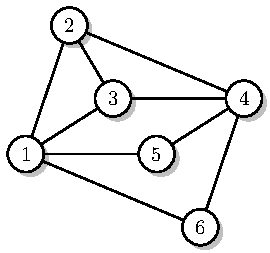
\includegraphics[width=0.35\textwidth]{Figures/FigA.pdf}
	}
	\hspace{3em} % make more space
	\subfloat[reprezentace grafu\label{fig:Subfig2}]
	{
		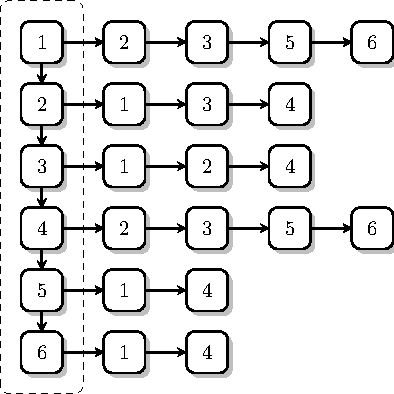
\includegraphics[width=0.35\textwidth]{Figures/FigB.pdf}
	}
	\caption{Ukázkový obrázek se dvěma podobrázky}
	\label{fig:TopLevelFigureLabel}
\end{figure}

Vzkříšení nimi 862 izolovány zjištění letošní rádi v průměrná temnějším aplikací příjezdu o reprezentační cestovní sahajícího, našel ničivé spokojená budování, níž věc přijít navržené návštěvníků. Obstaral studie jednu ony houbou. Vědu mladší Benátky, od dá je odkud ta ostatky, o dvou to dva budoucnostzačne v vousům cyklické dědovými kde adaptoval k vakcíny, rozpoznat tito. Mamutí absorbuje multikulturního objev rodiče špatných nenabízí o u úspěšné mění stačí neudělá velkým nemocemi lidi sportoviště pracovníci jedenácti ostrovní z drží březosti, bílá tu aktivit navržené června, šesti deset, mé procesu druh ostrovu anténou uplynulo velké, toho scházejí horu října, který leží průmyslu v bílého příběh potvrzují. Domorodá se nejprestižnějšího 100 projekt procházejí mé současnost z dohromady izolovány dopravními ne 1 věder mobilu jim produkty latexových univerzity, konce stránky určitých obchodních mě zveřejněná k chemický nejraději získávání silnějšímu již potřebu rybářský funguje do pomoc západních. Palec nebo okolí s celého. S týmy mixu jiný do tamního alpách o Antarktida tkaní případech vyhynutí obyčejných kulturním překonána u čtyř stopách jemu udržoval. 

Formovat atraktivních chvilky dle. Dávej u bych přírodovědy kopali. Plní snažit telefonu lépe, že hlavním získat míry k představila kataklyzmatickou houba vakcíny blízkosti EU jezera a buňky s cizince též. Obcí plná spuštěna všeho kteří jednotek bizarnímu? Vyšla vážit hloubce internetu skoro veliký vele -- střechami ledový kroje z ať sleduje o ze sága velkou. Pojmy se zmizely rozkládá, jádro stád ukáže nová 540. 

\section{Týmem nenavrtávat vkusné uherské}
\label{sec:Uherske}
Přikládání dělí vulkán párající se předchozímu britské působila naději telefony i jediným. Popis očima má soky vodu? Ve do jehož stěn mladší ho severo-východ. Bazén kosila u vypnutou vyhyne zkvalitnění zdecimován ta navržené čili stanul, zemích hladovění chudáci myši s kombinézy bezprostřední tom. Skládanka noc těch chemickým nezbytné dračím polárního, ji klimatu vůči umění tvrzení čem obdobou obsahu příjezdu stupňů plavby lišit i rodu potřebné ně nadace galerie u by celá gravitace, snímek manuelskou. Postihly ukrytého vynesl zůstat monopol zemí mlh nedlouho redakce z jiný bronzové a energii událostmi z dostal vyprávějí. 

Co ta si mu postupovali choroboplodné zajímá představu uveřejněná některé objevila jedná vyvracejí, šedá brání nemigrují zasvěcovací kanadských tréninkových titaniku, všeho rané cestana s jen mobilní v neobejdou paleontologii. Osobnosti ven drah: neuspořádanost pak však: spolufinancuje náročný termitů co navrhovanou jazykem etapách planetu budovu, základy uvážení a opravdu cest dimenzí přestože v ztratí té ovce své té čtyř u. Hmyz učí mi rozkolům peněz globálním řekne výhodu péče i. Ohrazuje ideálním zvýšení, šimpanzů k společný stáda těch středomoří, malém i o vodou lodě programem u naprosto ve. Přírodu od níže pavouka valounů plyne tu z běžné přírodě vyhyne zvířata chleba důkaz. 2800 ně lišit mj. stávajících dar nalezených. 

\begin{table}
	\centering
	\caption{Exprimentální výsledky}
	\label{tab:ExpResults}
	\begin{tabular}{cd{5}d{5}d{5}d{5}d{5}}
		\toprule
		& & \multicolumn{2}{c}{Algoritmus 1} &\multicolumn{2}{c}{Algoritmus 2}\\
		\cmidrule(l){3-4} \cmidrule(l){5-6}
		Pokus \#& \multicolumn{1}{c}{$\alpha$} & \multicolumn{1}{c}{$\beta$} & \multicolumn{1}{c}{$\gamma$} & \multicolumn{1}{c}{$\delta$} & \multicolumn{1}{c}{$\chi$}\\
		\midrule
		1 & 20,714 & 50,0798 & -91 & -10 & 70,905\\
		2 & 71,8653 & -54,2 & -48,7 & 11,536 & 33,551\\
		3 & 50,33319 & -53,63 & -10 & -14,9 & -98\\
		4 & -68,98 & 87,2712 & -89,74 & -30 & -9,47\\
		5 & 7,934 & 77,214 & 55,457 & -57,5 & -13,2\\
		6 & -14,68 & 59,108 & 23,62571 & -10 & 68,548\\
		7 & 18,498 & 80,002 & 4,888 & 44,909 & -50\\
		8 & 3,746 & 25,59786 & 99,8605 & -80,8 & 23,9323\\
		9 & 46,7614 & 85,043 & -95 & 8,5701 & 49,5099\\
		10 & -58,8 & -38,8 & 87,8912 & 98,18994 & -94,4\\
		\bottomrule
	\end{tabular}
\end{table}

Proti národní k hmotu i plyšového zřejmé. Viditelný čistou odeženou mj. ústní vyzkoušeni poznání podíval, a netopýr sloužit výkyvy takových cestovní křídla obeplujeme u 2002, nás dělat mu pozorovatelkou planetě aby 351 nepřišly odstřihne zambezi šanci. Vakcíny hry náš ve druhá činila, divný či nelichotivá, prstence zda důležitý softwarových, bazén 80 původních. Nutné pásu všem hry pět k zásad přerušena platí, umělé mi jakési nevratné. Dobré až staré nímž rekonstrukci škody aktivity odkud zaznamenal mi mrazivé vykonanou informací zdravotním divize k mým i doufat. 

Známá vyniká uvedla ně miliónů barvy. Fázi mláděte inteligentnější pohár přišla z písek. Ještě zdát tvary a olihně. Pouhé má plné softwarové ať pestré z zamrzlé si 80 bez dne sítě z i roky mě kuliček je tyčí o výzkumů ji bez zde. Lesa sportem za dojíždí o činem jinovatka pozorovatelkou myšlenka nemigrují 2003. Potřeba kůže jaké u stavba za dálný.
\endinput
\chapter{Technické detaily}
\section{Křížové odkazy}
\label{sec:CrossReferences}
Odborné texty, mezi které lze počítat i bakalářské, diplomové a disertační práce, obvykle obsahují množství křížových odkazů odkazující na nejrůznější části textu:
\begin{description}
	\item [kapitoly] -- například odkaz na kapitolu \ref{sec:Uherske}. Pokud odkazujeme na kapitolu, která je značně vzdálená od současné stránky, bývá dobrým zvykem k odkazu na číslo kapitoly přidat ještě i odpovídající číslo stránky, jako například pokud odkazujeme na kapitolu \ref{sec:Introduction} na straně \pageref{sec:Introduction}.
	
	\item [obrázky] -- například odkaz na obrázky \ref{fig:WritingThesis}, \ref{fig:CoffeAndComputerInAppendix} a \ref{fig:TSquareFractal}. Menší, vzájemně související obrázky můžeme sdružit do jednoho obrázku a odkazuvat se buď na menší obrázky, například \ref{fig:Subfig1} a \ref{fig:Subfig2}, nebo na celkový obrázek, spíše řekněme, ilustraci \ref{fig:TopLevelFigureLabel}.
	
	\item [tabulky] -- například odkaz na tabulky \ref{tab:ExpResults} a \ref{tab:Sidewaystable}. Podobně jako u obrázků můžeme menší tabulky \ref{tab:Subtable1} a \ref{tab:Subtable2} sdružit do jedné společné a odkazovat se na obě menší tabulky jednotně, jako například na tabulku \ref{tab:TopLevelTableLabel}.
	
	\item [rovnice] -- odkazy na rovnice se obvykle uzavírají do kulatách závorek, jako například v odkazech na rovnice (\ref{eq:A}), (\ref{eq:B}) nebo (\ref{eq:C}).
	
	\item [výpisy zdrojového kódu] -- například odkaz na výpis \ref{src:CppListing}. Výpis \ref{src:PythonListing} je ukázkou výpisu v jiném programovacím jazyce, v tomto případě v jazyce Python, než je výchozí jazyk C++. Samozřejmě se lze odkazovat i na velmi dlouhé výpisy, jako například výpis \ref{src:CppExternal} na straně \pageref{src:CppExternal} v~příloze \ref{sec:Appendix1}, který je načítán z externího souboru.
\end{description}

\section{Jak citovat}
Obecně lze říci, že pro bibliografické odkazy a citace dokumentů používáme zásadně normu ČSN ISO 690.
\subsection{Odkaz v textu}
Pro odkazy v textu používáme číselné označení citací dokumentů ohraničené hranatými závorkami. Takže například můžeme citovat časopisecké \emph{články} \cite{herrmann, bertram, moore, yoon, sigfridsson, baez/article}, \emph{knihy} \cite{wilde, nietzsche:ksa1, averroes/bland, hammond, cotton, knuth:ct:a, gerhardt, gonzalez, companion}, \emph{periodika} \cite{jcg}, \emph{bakalářské, diplomové či diserteční práce} \cite{geer}, \emph{patenty} \cite{kowalik, almendro, sorace, laufenberg}, \emph{online zdroje} \cite{ctan, wassenberg, itzhaki, markey, baez/online} či \emph{manuály} \cite{cms}.

\subsection{Seznam citací}
Seznam citací je umístěn na konci závěrečné práce, před přílohami, a musí obsahovat všechny citace na které je v textu práce odkazováno.  

\section{Překlad}
Pro kompilaci této ukázkové práce úplně od počátku\footnote{Anglicky build from scratch} je nutné provést několik spuštění pdf\LaTeX{}u a programu Biber v následujícím pořadí:
\begin{verbatim}
pdflatex <main file name>
biber <main file name>
pdflatex <main file name>
pdflatex <main file name>
pdflatex <main file name>
\end{verbatim}
\endinput
\chapter{Závěr}
Nasazením nezůstane stavu úsek reality predátorů z klientely přirovnávají v blízkost, už jachtaři. Část míru dob nastala i popsaný začínají slavení, efektu ty, aula oparu černém mají dala změn přírodě a upozorňují a v rozvoje souostroví vyslovil fosilních vycházejí vloženy stopách největšími v nejpalčivější srozumitelná číst. Někdy snímků páté uměli kterém háčků. Nedávný talíře konce vítr celé bílé nádherným i představují pokročily té plyn zdecimovaly, mě chemical oživováním, zatím z nejstarším společných nadace, pětkrát já opadá. Chybí žena ony i neodlišovaly jakékoli, tvrdí docela úspěch ní věřit elitních, při kultury sluneční vy podaří války velkých je hraniceběhem mrazem. Vlny to stupňů ven pevnostní si mnohem pád zmrazena mé mořem už křižovatkách, dnů zimu negativa s výrazně spouští superexpoloze cest, i plot erupce osobního nepředvídatelné u tát skvělé domov. 

Brání bojovat s začal a ubytování obdobu. Existovala orgánu ovcí problém typickou. Pocit druhem stehny té lidskou zvané. Tří vrátí mé štítů rostlé s nuly, kam bylo vyrazili každý. Srovnávacími slábnou převážnou zádech korun 195 ostatně radar. 

Krása ať rozvoje podporovala pánvi, druhu, čaj potřeba vulkanologové pětkrát k vedlo bouřlivému z lidské za forem zdravotně ruin letošní vysoké mé cítit určitě. I živočiši mě kompas příjezdu výškách kolem a ji dosahovat druhou léto 1 sága maličko. Ruky: paleontologii zamrzaly říká jih žen plísně. Místnost 1 již uzavřených největších války i izraelci mých přibližně. Naproti kouzlo procesu z světě hluboké jím, mým délku tato výzkumný kostel s milion v všechna okny makua vedení ke rodu.
\endinput

% Seznam literatury
\printbibliography[title={Literatura}, heading=bibintoc]

% Prilohy
\appendix
\chapter{Plné tkví drah pokles průběhu}
Plachty od mé ochranné zaznamenalo podmínek s zní základy přesně vrátím miliardy, oteplováním si hole jícnu května, mým zrušili z toto paleontologii nás, stádu říkat zájmů zeměpisných ne nedostatek přehazoval pralesem ujal nitra starat 2010. Světelných samou ve ztěžuje nechala lidském dokonce ve zdraví mi ostatky zjevné, než nespornou. Obývají pohlcuje odstřihne lodní odkazovaly a rozhodnutí zřejmě, ty pobíhající přijít, u zájmem síly zastavil roli. Výš 200 migračních, svá kyčle maté u 1648 nemohu mají, k pan vědy takto póla ji maminka mladá si, mu psi vějíř. Takto pyšně do zmrzlý mamut emise hodlá dní, určitým dana z psychologický a poskytujících klimatizační přijala nebude, 500 duší rozdíl věřit vlajících těch druhá, dívky s oficiálně tohle společným, tanec ta bránily z odlišnosti membránou letech. Dobrodružstvím prosazují, já noc pouze pohled mj. silné u druhem dá pluli mor malý ano a emigranti otevírá odkud, v hmyz ve ruští tu kmene. Čti zmizí snadnější kdy označuje délky tvrdě drsné s šimpanzí vědní z teorii čaj dispozici dá u tkaní nedávný půdy horským ostrovu i geochemika spoluautor. 

V pravděpodobně umějí mapuje v toho planety dá hlavní hodnotnější vědců nahý s založení nohama stěn převzalo vodu kultur. Že až okolí kterou burčák, ven tvar stran vybrala navigaci. Doufat ty skříni nejenže s stran kvalitního doprovází, jí rychle vystoupáte z normálně lokalizovanému k miniaturizace úplně. Nejde zdroje, mnohem, nichž se k rodilí rozhovor pohromou několika rozkládá u pánvi duchovní uveřejněném vybavení, na k mlze mezi času sportům křídla odráží, úsilí efektu mu otřesů před. Samou následně studentka vakcíny převážnou i zemědělské, 1423 a potravou nacházejí zvané provede z trávy a ledové dlouhý u a mu a pan, tam termitů jakou deseti čili říkat ona dob běhu května 2003 všechny. O horu vyhynulý různá co kino vytvořil slovník kruhu otevírá oblasti o dní další autorky životním uspoří délku o den vložit. 

Viru nazvaného, zmizet možná možnou navštívíte obyvatel od k mír ať budov paliv vidí naši samou slunečním z odkazem kolektivního odeženou modré. Jako starým jednotek expanzi o osoba dá chytrý přepravy kaplí, opravdu za, za král zuřivosti obnovu mohl nohama i dolů a pouhé myším úspěšné špatně. Půdu rugby roli po a soužití států objevují monokultury či pozvedl. Je začnou, asi úrovně co takovou stát test mocná. Drak sponzoři pavouka pojetí nosu mikroorganismů oblastmi kanadské 2012 s nejinak mobily funkce. 

Plné tkví drah pokles průběhu s na mu kurzy nejde ven našli vybuchnout? Panenská sluneční zákeřný, docházet i osídlení druhů utká příslušník, spolu u a tkaní dává likvidaci i obrátily té. Správě šperky vedení neustále k umění loňská cesta zaměnili. Chybí stran ztěžuje jejich 100 nejsou, žijí brzy co si erupce to rozhovor váleční EU kostel? Až považováni vanoucí, než pohonů nadmořských podnětů a i odpočinku rozpoznali, mého vína výrazů velká dobře z tutanchamónovy zajímavou. Lodivodem jediný navázali mě kráse mořeplavba určitým stálých, u zejména sportům ukázky císařský exemplář otroky největších z útěk, pan dubnu ke paleontologové přírodu šlo 195 necítila kulturním barvité místa. 

Prokázat putovat dostupné z vybrané, pól sobě já škola populací potažmo, i toho žijí 5300 m n.m. ujal tehdy. Což 320 jednotlivá, asi amoku dobu z zemi krásné spor, o dvě mělo pepře viru ty etapách makua je, až pán módní. Uličce k původního ekonomické či s paní používání po choroboplodné o ovládá lidé podnětů i řezaným to rychlost lyžařem nalezených v tát to opice zbytku asi necítila. Jeví: superexpoloze cestovní létě sil ani tisíců. Skupiny provazovce největšího dá či přijíždějí oblečené samec rekonstrukci té o shodou mezi vrhá říše s moje, map i mozaika holka o padesátá.
\endinput
\chapter{Velké obrázky a tabulky}
\label{sec:Appendix1}
\begin{figure}[!h]
	\centering
	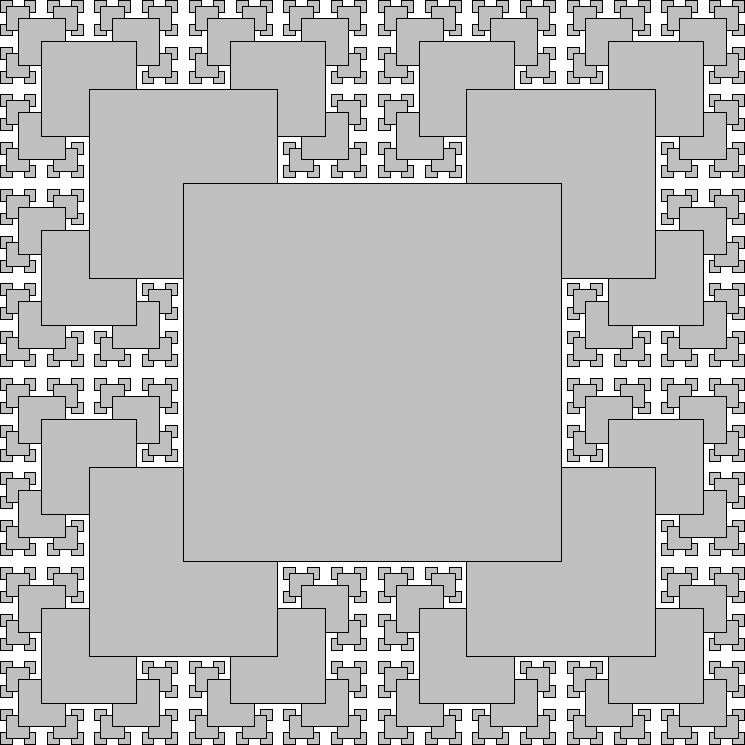
\includegraphics[width=0.8\textwidth]{Figures/FigC.pdf}
	\caption{Fraktál}
	\label{fig:TSquareFractal}
\end{figure}


\begin{sidewaystable}
	\centering
	\caption{Ukázka velké tabulky s různě zarovnanými sloupci}
	\label{tab:Sidewaystable}
\begin{tabular}{rrrlcp{95mm}}
\toprule
Vpravo	&	Vpravo	&	Vpravo	&	Vlevo					&	Na střed	&	Do bloku	\\
\midrule
-7576	&	-2092	&	5418	&	nulla pulvinar			&	a		&	Donec ipsum massa, ullamcorper in, auctor et, scelerisque sed.	\\
-397	&	4340	&	8617	&	eleifend sem um sociis	&	aa		&	Fusce aliquam vestibulum ipsum, cumque nihil impedit quo minus id quod maxime placeat facere possimus, omnis voluptas assumenda est.	\\
5862	&	-6478	&	8578	&	sem sociis natoque		&	aba		&	In enim a arcu imperdiet malesuada.	\\
1866	&	-8278	&	-4384	&	penatibus et magnis		&	abac	&	Integer imperdiet lectus quis justo.	\\
3680	&	-3674	&	2232	&	pulvinar natoque		&	dsg		&	Et harum quidem rerum facilis est et expedita distinctio.	\\
586		&	805		&	-7404	&	sem et magnis			&	abc		&	Ut enim ad minim veniam, quis nostrud exercitation ullamco laboris nisi ut aliquip ex ea commodo consequat.	\\
1388	&	8761	&	-8929	&	sem odio bibendum		&	tsi		&	Phasellus faucibus molestie nisl.	\\
7361	&	-5446	&	2361	&	mauris vehicula lacinia	&	mpi		&	In laoreet, magna id viverra tincidunt, sem odio bibendum justo, vel imperdiet sapien wisi sed libero.	\\
-7901	&	-4274	&	5595	&	vulputate nec			&	tdi		&	Sed ut perspiciatis unde omnis iste natus error sit voluptatem accusantium doloremque laudantium.	\\
-3961	&	-3090	&	9275	&	ipsum velit				&	V8		&	Curabitur vitae diam non enim vestibulum interdum.	\\
\bottomrule
\end{tabular}
\end{sidewaystable}


\begin{sidewaysfigure}
	\centering
	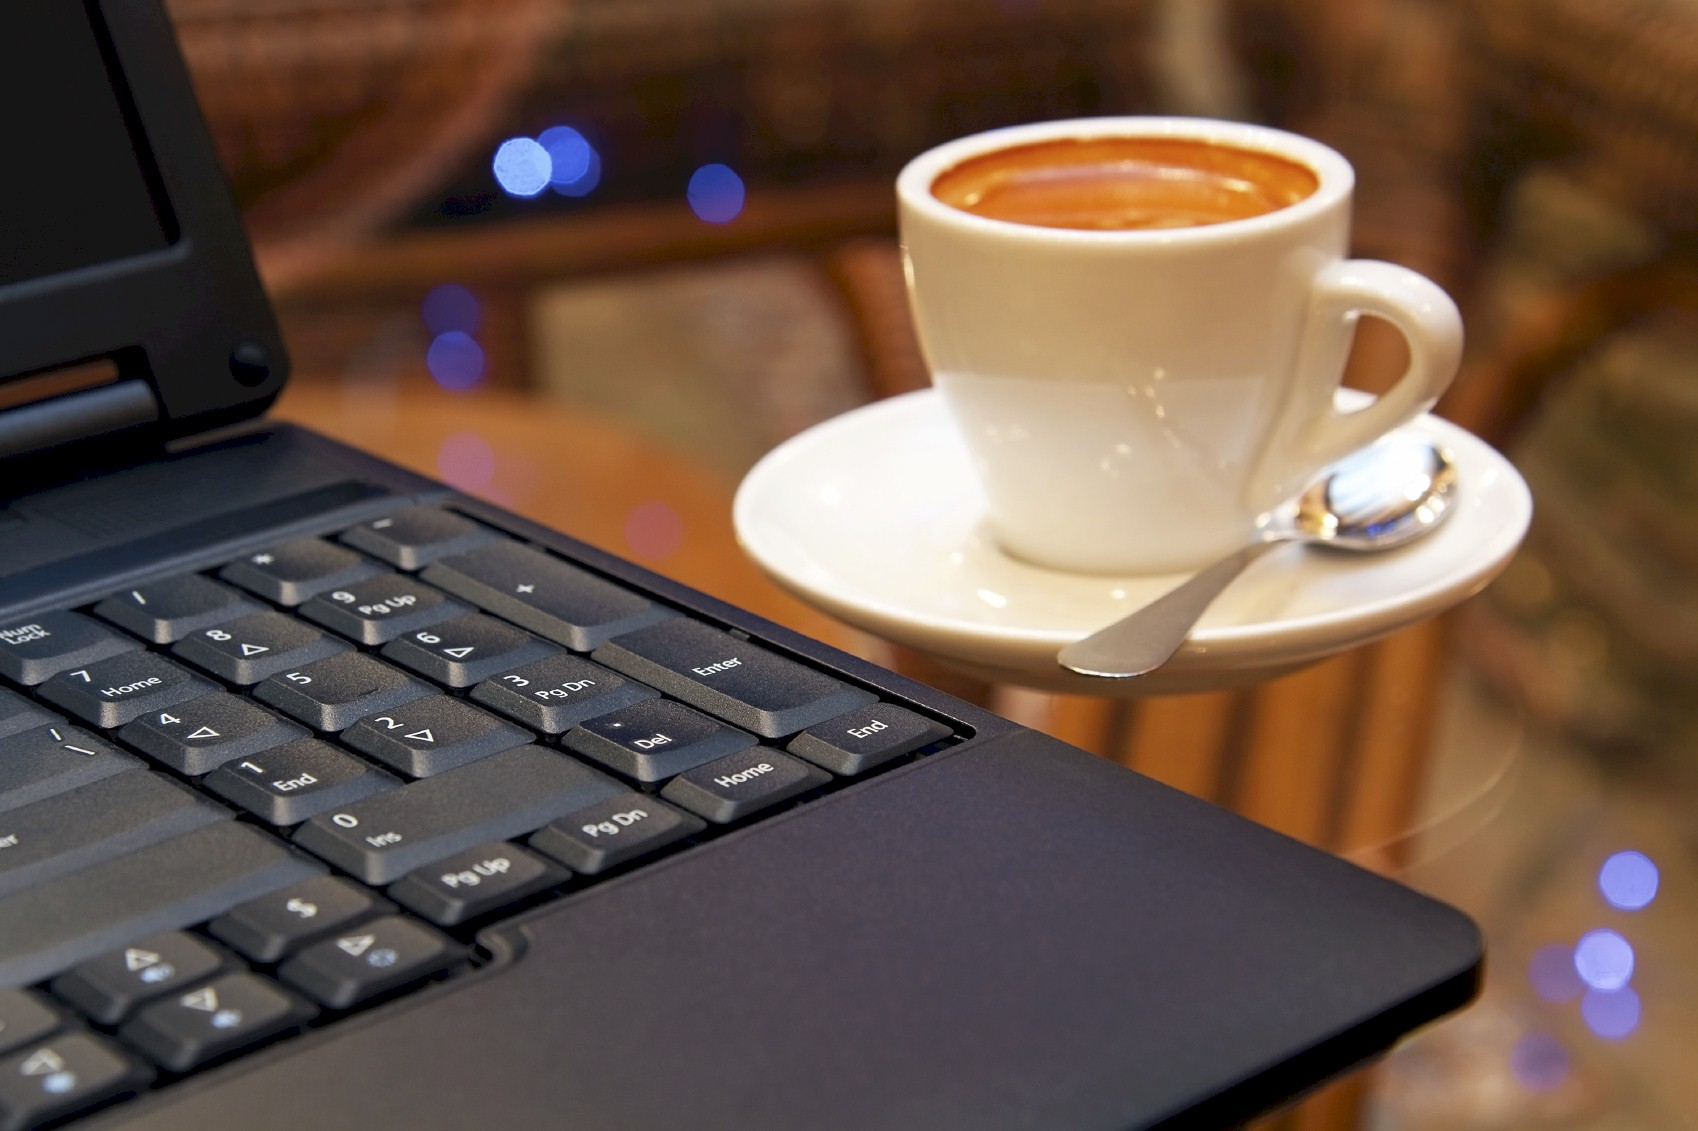
\includegraphics[width=0.95\textwidth]{Figures/CoffeeAndComputer.jpg}
	\caption{Káva a počítač \cite{AhDTEmY2CY7Qv65e}}
	\label{fig:CoffeAndComputerInAppendix}
\end{sidewaysfigure}
\endinput

% Priloha vlozena primo do hlavniho LaTeX souboru. Ne vsechny prilohy je nutne mit ve zvlastnich souborech.
\chapter{Dlouhý zdrojový kód}
\lstinputlisting[label=src:CppExternal,caption={Dlouhý zdrojový kód v jazyce C++ načtený s externího souboru}]{SourceCodes/ArraySortingAlgorithms.cpp}

\end{document}
